\section{Optimizaciones}

Las optimizaciones se han llevado a cabo sobre las funciones
\texttt{electric\_field} y \texttt{pythagoras}.

Las optimizaciones se han realizado de forma incremental. Esto significa que la
optimizaci\'{o}n X incluye las optimizaciones 0 a X-1 y que las modificaciones
se han realizado sobre la versi\'{o}n X-1.

El an\'{a}lisis de rendimiento de una optimizaci\'{o}n se ha hecho comparando
con la optimizaci\'{o}n anterior y con el c\'{o}digo de base. Con estas dos
comparaciones se puede observar cual es la aceleraci\'{o}n de la optimizaci\'{o}n
propuesta y cual es la aceleraci\'{o}n total acumulada, respectivamente.

\subsection{Opt1: Evitar llamadas a funciones}

Las llamadas a funciones son un tipo de instrucci\'{o}n costosa que conviene
evitar siempre que sea posible. Algunas de las t\'{e}cnicas m\'{a}s comunes
para evitar llamadas a funciones son el inlining, la memorizaci\'{o}n o la
substituci\'{o}n de la llamada por un valor igual al valor de retorno.
\'{E}sta \'{u}ltima t\'{e}cnica es la que se puede utilizar para evitar llamar
a la funci\'{o}n \texttt{gaddress}.

La funci\'{o}n \texttt{gaddress} se encarga de calcular un \'{i}ndice de un
vector a partir de los cuatro par\'{a}metros que recibe. En el c\'{o}digo de
\texttt{electric\_field} se llama a la funci\'{o}n \texttt{gaddress} en
muchas ocasiones de forma innecesaria. La llamada es innecesaria porque la
secuencia de valores de retorno que generan las llamadas a \texttt{gaddress}
en el c\'{o}digo original es 0, 1, 2, ..., grid\_size-1, grid\_size+2,
grid\_size+3, etc. El c\'{o}digo original es el siguiente:

\begin{lstlisting}[]
     for( x = 0 ; x < grid_size ; x ++ ) {
        for( y = 0 ; y < grid_size ; y ++ ) {
           for( z = 0 ; z < grid_size ; z ++ ) {
              grid[gaddress(x,y,z,grid_size)] = ...
           }
        }
     }
\end{lstlisting}

La optimizaci\'{o}n propuesta consiste en cambiar la llamada a
\texttt{gaddress} por un simple contador que se incrementa en uno en cada
iteraci\'{o}n sobre \texttt{z} y en dos en cada iteraci\'{o}n sobre
\texttt{y}, generando as\'{i} los \'{i}ndices correctamente. El c\'{o}digo
resultante es el siguiente:

\begin{lstlisting}[]
     i = 0;
     for( x = 0 ; x < grid_size ; x ++ ) {
        for( y = 0 ; y < grid_size ; y ++ ) {
           for( z = 0 ; z < grid_size ; z ++ ) {
              grid[i] = ...
              i++;
           }
           i += 2;
        }
     }
\end{lstlisting}

Esta optimizaci\'{o}n se ha aplicado de la misma forma en otros puntos, como en
\texttt{electric\_field\_zero\_core} o en el primer bucle de
\texttt{electric\_point\_charge}.

La siguiente gr\'{a}fica muestra los tiempos de ejuci\'{o}n de la versi\'{o}n
original y de la versi\'{o}n Opt1.

\begin{figure}[ht]
   \centering
   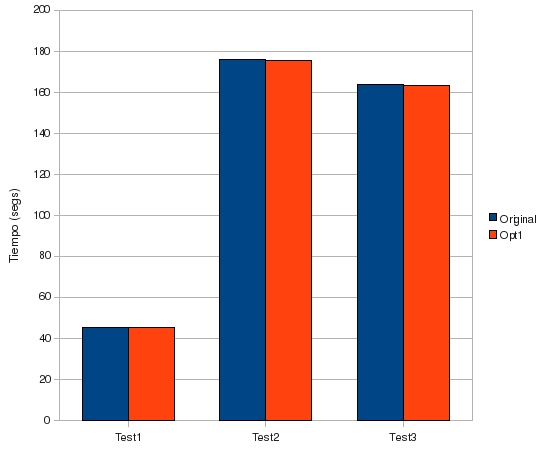
\includegraphics[keepaspectratio=true,width=.5\textwidth]{figures/opt1-perf}
\end{figure}

Para el primer test la aceleraci\'{o}n es del 0.288\%, para el segundo es del
0.149\% y para el tercero es del 0.272\%.

Como se puede observar, la aceleraci\'{o}n que se consigue es m\'{i}nima. El
motivo es que esta parte del c\'{o}digo tiene poco peso en el tiempo de
ejecuci\'{o}n ya que se encuentra fuera del bucle m\'{a}s interno del programa.
Adem\'{a}s la funci\'{o}n \texttt{gaddress} es en realidad una macro bastante
simple.

\subsection{Opt2: Filtrado de datos}

Filtrar datos es una t\'{e}cnica que permite reducir el tama\~{n}o de datos a
tratar. Los efectos son muy beneficiosos si el c\'{o}digo computa una serie de
datos de una forma y otra serie de datos de otra forma. El filtrado de datos se
suele acompa\~{n}ar de otras t\'{e}cnicas como la compactaci\'{o}n de dichos
datos o la eliminaci\'{o}n de condicionales.

La primera l\'{i}nea del cuerpo del bucle m\'{a}s interno de
\texttt{electric\_field} es una comprobaci\'{o}n que hace que sobre un
subconjunto de datos se ejecute el cuerpo del bucle y sobre otro subconjunto no
se haga nada.

\clearpage

\begin{lstlisting}[]
     for( atom = 1 ; atom <= This_Structure.Residue[residue].size ; atom ++ ) {
        if( This_Structure.Residue[residue].Atom[atom].charge != 0 ) {
           distance = pythagoras( This_Structure.Residue[residue].Atom[atom].coord[1] ,
                                  This_Structure.Residue[residue].Atom[atom].coord[2] ,
                                  This_Structure.Residue[residue].Atom[atom].coord[3] ,
                                  x_centre , y_centre , z_centre ) ;
           ...
        }
     }
\end{lstlisting}

Aplicando esta condici\'{o}n a un proceso de filtrado se puede evitar hacer la
comparaci\'{o}n dentro del cuerpo del bucle, que puede llegar a ser muy costoso.
Adem\'{a}s el filtrado se puede aprovechar para compactar los valores que se van
a utilizar de \texttt{This\_Structure.Residue[residue].Atom[atom].charge} y de
\texttt{This\_Structure.Residue[residue].Atom[atom].coord} en vectores
auxiliares. El c\'{o}digo del filtrado y la modificaci\'{o}n del bucle son los
siguientes:

\begin{lstlisting}[]
    indexCoord = 0;
    indexCharge = 0;
    for( residue = 1 ; residue <= This_Structure.length ; residue ++ ) {
       for( atom = 1 ; atom <= This_Structure.Residue[residue].size ; atom ++ ) {
          if( This_Structure.Residue[residue].Atom[atom].charge != 0 ) {
             charge[indexCharge] = This_Structure.Residue[residue].Atom[atom].charge;
             coord[indexCoord]   = This_Structure.Residue[residue].Atom[atom].coord[1];
             coord[indexCoord+1] = This_Structure.Residue[residue].Atom[atom].coord[2];
             coord[indexCoord+2] = This_Structure.Residue[residue].Atom[atom].coord[3];
             indexCharge++;
             indexCoord+=3;
          }
       }
    }
    ....
    for( atom = 0 ; atom < indexCharge ; atom ++ ) {
       distance = pythagoras(coord[indexCoord],coord[indexCoord+1],coord[indexCoord+2],
                             x_centre,y_centre,z_centre) ;
       ...
    }
\end{lstlisting}

La siguiente gr\'{a}fica muestra los tiempos de ejuci\'{o}n de la versi\'{o}n
original, de la versi\'{o}n Opt1 y de la versi\'{o}n Opt2.

\begin{figure}[ht]
   \centering
   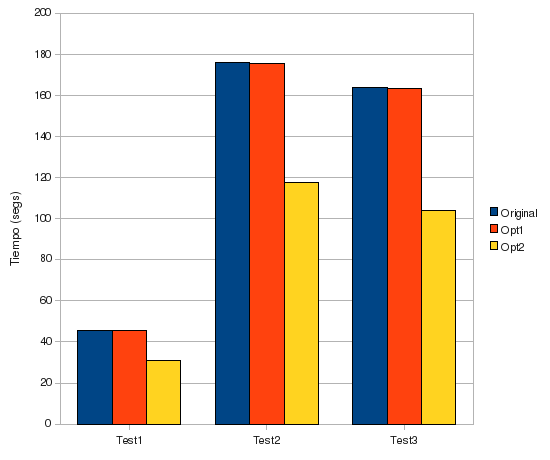
\includegraphics[keepaspectratio=true,width=.5\textwidth]{figures/opt2-perf}
\end{figure}

Las aceleraciones acumuladas sobre la versi\'{o}n original son del 47.742\% para
el primer test, 49.806\% para el segundo test y 57.548\% para el tercer test.
Sobre la versi\'{o}n Opt1 las aceleraciones son del 47.317\%, 49.583\% y 57.1197\%
para el primer test, el segundo y el tercero, respectivamente.

Como se puede observar, la aceleraci\'{o}n que se consigue es muy grande, ya que
el filtrado permite optimizar el cuerpo del bucle m\'{a}s interno del programa,
que se ejecuta muchas veces.

\subsection{Opt3: Evitar saltos}

Los saltos, como las llamadas a funciones, son instrucciones que pueden llegar
a ser muy costosas debido a  los posibles fallos del predictor de saltos, por
eso es conveniente evitar los saltos innecesarios.

En el bucle m\'{a}s interno de la funci\'{o}n \texttt{electric\_field} hay
varias comprobaciones que se traducen en saltos al compilar. Algunas de estas
comprobaciones son innecesarias u optimizables.

\begin{lstlisting}[]
     if( distance < 2.0 ) distance = 2.0 ;
     if( distance >= 2.0 ) {
        if( distance >= 8.0 ) {
           epsilon = 80 ;
        } else {
           if( distance <= 6.0 ) {
              epsilon = 4 ;
           } else {
              epsilon = ( 38 * distance ) - 224 ;
           }
        }
        phi += ( (charge[atom]) / ( epsilon * distance ) ) ;
     }
\end{lstlisting}

La segunda comprobaci\'{o}n se puede eliminar ya que siempre se cumple debido a
la asignaci\'{o}n de la l\'{i}nea anterior. Adem\'{a}s, la secuencia de
condicionales imbricados para asignar un valor a \texttt{epsilon} se puede
simplificar. El c\'{o}digo resultante es:

\begin{lstlisting}[]
     if( distance < 2.0 ) distance = 2.0 ;
     if (distance >= 8.0)
        epsilon = 80;
     else if (distance <= 6.0)
        epsilon = 4;
     else
        epsilon = 38 * distance - 224;
     phi += ( (charge[atom]) / ( epsilon * distance ) ) ;
\end{lstlisting}

Otra fuente de saltos innecesarios es el primer bucle de la funci\'{o}n
\texttt{electric\_field}. El c\'{o}digo original es:

\begin{lstlisting}
     i = 0;
     for( x = 0 ; x < grid_size ; x ++ ) {
        for( y = 0 ; y < grid_size ; y ++ ) {
           for( z = 0 ; z < grid_size ; z ++ ) {
              grid[i] = (fftw_real)0;
              i++;
           }
           i += 2;
        }
     }
\end{lstlisting}

Como se puede observar, los bucles sobre \texttt{x} e \texttt{y} se pueden
fusionar en uno solo y as\'{i} evitar un salto. El resulado es el siguiente
c\'{o}digo:

\begin{lstlisting}
     i = 0; 
     j = 0;
     while( j < grid_size*grid_size*grid_size) {
        for( i = j ; i < j+grid_size ; i ++ ) {
           grid[i] = (fftw_real)0;
        }
        j += grid_size + 2;
     }
\end{lstlisting}

Esta optimizaci\'{o}n se ha aplicado de la misma forma en otros puntos, como en
\texttt{electric\_field\_zero\_core} o en el primer bucle de
\texttt{electric\_point\_charge}.

La siguiente gr\'{a}fica muestra los tiempos de ejuci\'{o}n de la versi\'{o}n
original, de la versi\'{o}n Opt2 y de la versi\'{o}n Opt3.

\begin{figure}[ht]
   \centering
   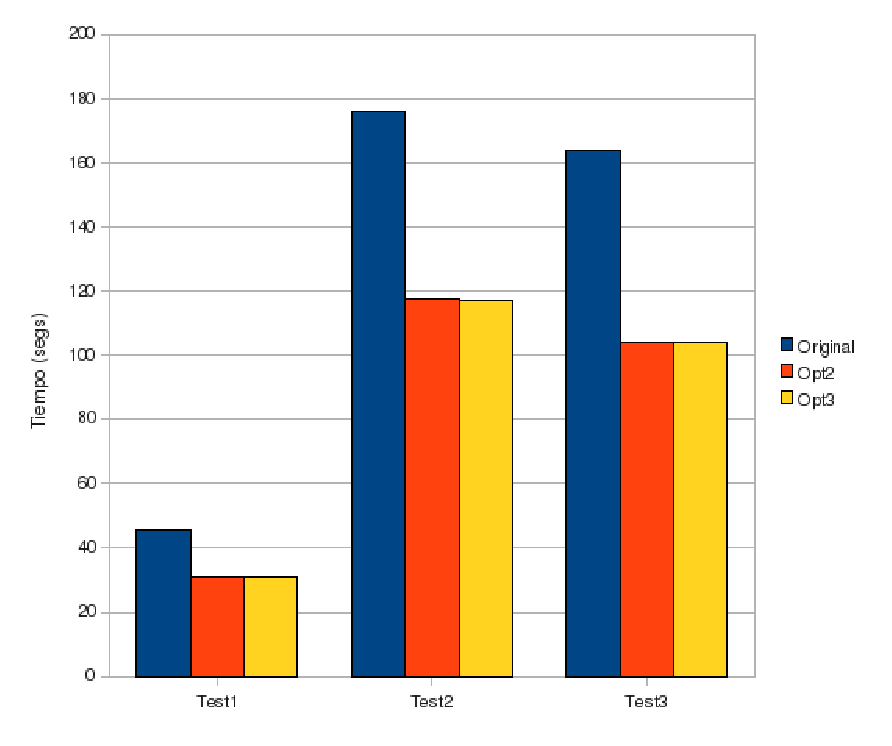
\includegraphics[keepaspectratio=true,width=.5\textwidth]{figures/opt3-perf}
\end{figure}

Las aceleraciones acumuladas sobre la versi\'{o}n original son del 48.001\% para el
primer test, 49.983\% para el segundo test y 57.682\% para el tercer test. Sobre
la versi\'{o}n Opt2 las aceleraciones son del 0.175\%, 0.117\% y 0.085\% para el
primer test, el segundo y el tercero, respectivamente.

Como se puede observar, la aceleraci\'{o}n que se consigue es m\'{i}nima. El
motivo es que el condicional que se ha quitado del cuerpo del bucle m\'{a}s
interno ya lo optimizaba el compilador y la optimizaci\'{o}n de los
\texttt{if-then-else} no simplifica mucho las condiciones.

\subsection{Opt4: Evitar llamadas a sistema}

Las llamadas a sistema son un tipo de instrucci\'{o}n especialmente costoso, ya
que provocan tener que entrar a modo sistema, salvar el contexto, ensuciar la
cache, etc. La tecnica m\'{a}s utilizada para evitar llamadas a sistema es el
buffering, o juntar varias llamadas a sistema en una.

En cada iteraci\'{o}n del bucle m\'{a}s externo del cuerpo de
\texttt{electric\_field} se hace un \texttt{printf(".")}. Esto provoca que
la ejecuci\'{o}n se hagan \texttt{grid\_size} \texttt{printf}'s que escriben un
solo punto, cuando lo \'{o}ptimo es hacer un solo \texttt{printf} que escriba
\texttt{grid\_size} puntos.

\begin{figure}[ht]
   \centering
   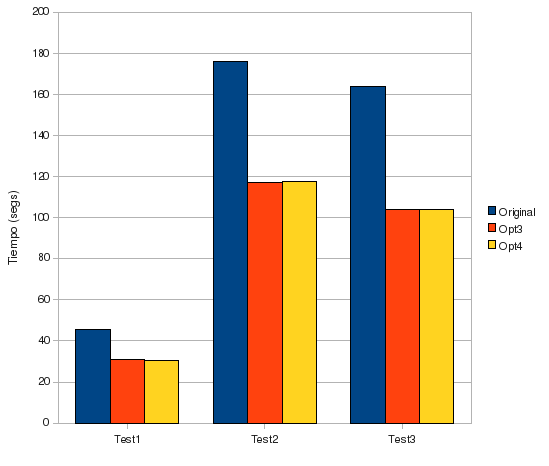
\includegraphics[keepaspectratio=true,width=.5\textwidth]{figures/opt4-perf}
\end{figure}

La gr\'{a}fica anterior muestra los tiempos de ejuci\'{o}n de la versi\'{o}n
original, de la versi\'{o}n Opt3 y de la versi\'{o}n Opt4.

Las aceleraciones acumuladas sobre la versi\'{o}n original son del 48.325\% para el
primer test, 49.856\% para el segundo test y 57.828\% para el tercer test. Sobre
la versi\'{o}n Opt3 las aceleraciones son del 0.218\% y 0.092\% para el primer
test y el tercero, respectivamente. Para el segundo test hay una
desaceleraci\'{o}n del 0.085%.

Como se puede observar, la aceleraci\'{o}n que se consigue es m\'{i}nima. El
motivo es que el peso de las llamadas a sistema en el tiempo de ejecuci\'{o}n
es muy peque\~{n}o ya que la llamada se encuentra en el bucle m\'{a}s externo.

\subsection{Opt5: Unrolling}

El unrolling es una t\'{e}cnica que consiste en replicar el c\'{o}digo de un
bucle N veces para as\'{i} reducir el n\'{u}mero de saltos que se realizan al
ejecutar el c\'{o}digo de control del bucle. El n\'{u}mero de saltos se divide
por N.

En el c\'{o}digo original el bucle m\'{a}s interno se hace de esta forma:

\begin{lstlisting}
     for( atom = 1 ; atom <= indexCharge ; atom ++ ) {
        cuerpo
     }
\end{lstlisting}

El unrolling realizado es de grado 4, es decir, se replica el cuerpo 4 veces y
se incrementa la variable \texttt{atom} en 4 en vez de en 1. Puede pasar que el
n\'{u}mero de iteraciones no sea divisible por 4, por eso hay que dividir el
bucle en dos. En el primero se ejecutan tantas iteraciones como se puedan en
grupos de 4 iteraciones, mientras que en el segundo se ejecutan el resto de
iteraciones. El c\'{o}digo resultante es el siguiente:

\begin{lstlisting}
     num_unrolled_iters = indexCharge - (indexCharge % 4);
     for( atom = 0 ; atom <= num_unrolled_iters ; atom += 4 ) {
        cuerpo0
        cuerpo1
        cuerpo2
        cuerpo3
     }
     for( atom ; atom <= indexCharge ; atom ++ ) {
        cuerpo
     }
\end{lstlisting}

La siguiente gr\'{a}fica muestra los tiempos de ejuci\'{o}n de la versi\'{o}n
original, de la versi\'{o}n Opt4 y de la versi\'{o}n Opt5.

\begin{figure}[ht]
   \centering
   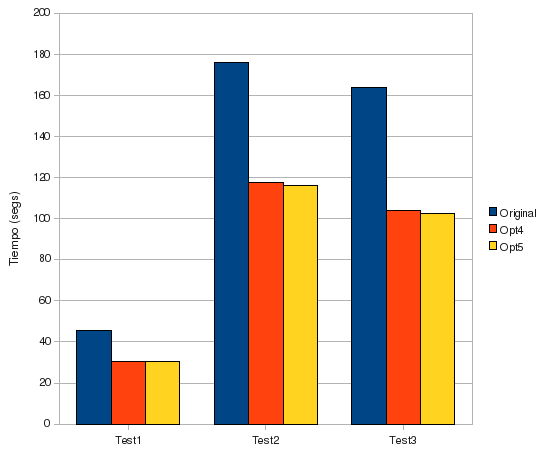
\includegraphics[keepaspectratio=true,width=.5\textwidth]{figures/opt5-perf}
\end{figure}

Las aceleraciones acumuladas sobre la versi\'{o}n original son del 49.942\% para el
primer test, 51.213\% para el segundo test y 59.945\% para el tercer test. Sobre
la versi\'{o}n Opt4 las aceleraciones son del 1.090\%, 0.905\% y 1.341\% para el
primer test, el segundo y el tercero, respectivamente.

Como se puede observar, la aceleraci\'{o}n que se consigue es m\'{i}nima. El
motivo es que se han reducido el n\'{u}mero de saltos, pero los saltos que se han
evitado eran muy predecibles para el predictor de saltos.

\subsection{Opt6: Vectorizaci\'{o}n}

La vectorizaci\'{o}n es una t\'{e}cnica que permite realizar una misma
operaci\'{o}n sobre diversos datos a la vez, dividiendo el tiempo dedicado a
hacer dichas operaciones por cierto factor. Esta t\'{e}cnica es aplicable
gracias a la existencia de registros vectoriales, que son registros f\'{i}sicos
de 16 bytes situados dentro del procesador.

FTDock trabaja sobretodo con floats, as\'{i} que al pasar el c\'{o}digo a vectorial
la t\'{e}cnica a seguir es cargar cuatro valores en un registro vectorial,
operar y volcar los cuatro resultados a memoria. Se utilizan cuatro valores
porque en un registro vectorial de 16 bytes caben 4 floats de 4 bytes cada uno.

En el bucle desarrollado mediante unrolling es trivial aplicar vectorizaci\'{o}n.
Lo que se ha hecho es cargar cuatro valores del vector \texttt{charge} en un
registro vectorial, calcular los coeficientes a partir \texttt{epsilon} y
\texttt{distance} en un vector y cargar ese vector en un registro vectorial para
poder hacer las cuatro divisiones a la vez. La suma con \texttt{phi} tambien se
hace vectorialmente, haciendo una operaci\'{o}n de reducci\'{o}n al final del
bucle. El c\'{o}digo resultante es:

\begin{lstlisting}
    for( atom = 0 ; atom <= num_unrolled_iters ; atom += 4 ) {
       atomVect = _mm_load_ps(&(charge[atom]));
       // Calculo de coeficientes en coefficient
       coefficientVect = _mm_load_ps(coefficient);
       atomVect = _mm_div_ps(atomVect,coefficientVect);
       phiVect = _mm_add_ps(phiVect,atomVect);
    }
    _mm_store_ps(phi,phiVect);
    phi[0] = phi[0] + phi[1] + phi[2] + phi[3];
\end{lstlisting}

La siguiente gr\'{a}fica muestra los tiempos de ejuci\'{o}n de la versi\'{o}n
original, de la versi\'{o}n Opt5 y de la versi\'{o}n Opt6.

\begin{figure}[ht]
   \centering
   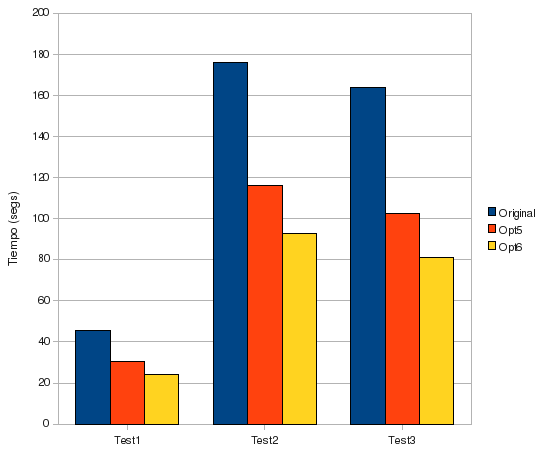
\includegraphics[keepaspectratio=true,width=.5\textwidth]{figures/opt6-perf}
\end{figure}

Las aceleraciones acumuladas sobre la versi\'{o}n original son del 87.628\% para el
primer test, 89.721\% para el segundo test y 102.424\% para el tercer test. Sobre
la versi\'{o}n Opt5 las aceleraciones son del 25.134\%, 25.466\% y 26.558\% para el
primer test, el segundo y el tercero, respectivamente.

Como se puede observar, la aceleraci\'{o}n que se consigue es muy importante. El
motivo es que muchos de los c\'{a}lculos se hacen en paralelo, lo cual reduce
mucho el tiempo de ejecuci\'{o}n.

\subsection{Opt7: Vectorizaci\'{o}n}

En la funci\'{o}n \texttt{pythagoras} se calcula la distancia eucl\'{i}dea
entre dos vectores. Para calcularla se ejecutan muchas instrucciones: se restan
de componentes, se hacen tres exponencial cuadradas, se suman todas las
componentes y finalmente se hace una raiz cuadrada del resultado de la suma.

\begin{lstlisting}
    sqrt(((x1-x2)*(x1-x2)) + ((y1-y2)*(y1-y2)) + ((z1-z2)*(z1-z2)));
\end{lstlisting}

La transformaci\'{o}n de esta funci\'{o}n a c\'{o}digo vectorial es inmediata:

\begin{lstlisting}
    __m128 v1 = _mm_set_ps(x1, y1, z1, 0);
    __m128 v2 = _mm_set_ps(x2, y2, z2, 0);
    v1 = _mm_sub_ps(v1, v2);
    v1 = _mm_mul_ps(v1, v1);
    _mm_storeu_ps(vector, v1);
    sqrt(vector[1]+vector[2]+vector[3]);
\end{lstlisting}

Como se puede ver en el codigo anterior, a la hora de cargar los valores al
registro vectorial hay que rellenar la \'{u}ltima posici\'{o}n con alg\'{u}n
valor aunque no se vaya a utilizar.

La siguiente gr\'{a}fica muestra los tiempos de ejuci\'{o}n de la versi\'{o}n
original, de la versi\'{o}n Opt6 y de la versi\'{o}n Opt7.

\begin{figure}[ht]
   \centering
   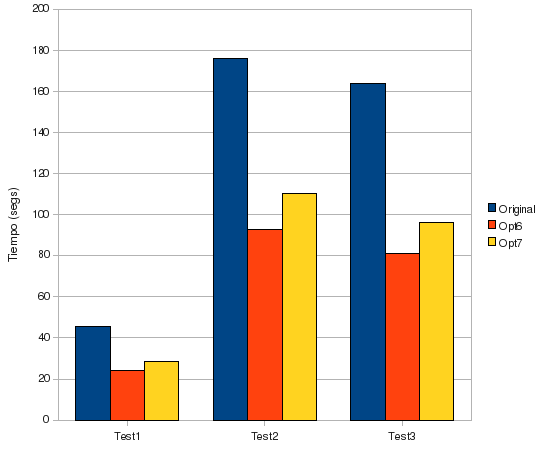
\includegraphics[keepaspectratio=true,width=.5\textwidth]{figures/opt7-perf}
\end{figure}

Como se puede observar, la optimizaci\'{o}n hace que el c\'{o}digo vaya m\'{a}
lento. En este c\'{o}digo solo se hacen dos operaciones vectoriales, una suma y
una multiplicaci\'{o}n, adem\'{a}s de solo utilizar tres de los cuatro valores
disponibles en el registro vectorial. Estos dos motivos, junto con que para
trabajar con vectores se necesita hacer un load hacia el registro vectorial y
un store a memoria, hacen que el rendimiento empeore.

\subsection{Opt8: Vectorizaci\'{o}n con SSE3}

Para intentar solventar el problema del coste que tiene hacer un load y un store
a un registro vectorial para hacer solo dos operaciones se han a\~{n}adido
m\'{a}s operaciones vectoriales y se han eliminado los accesos a memoria
utilizando intr\'{i}nsicas de SSE3.

\begin{lstlisting}
    float result;
    __m128 v1 = _mm_set_ps(x1, y1, z1, 0);
    __m128 v2 = _mm_set_ps(x2, y2, z2, 0);
    v1 = _mm_sub_ps(v1, v2);
    v1 = _mm_mul_ps(v1, v1);
    v1 = _mm_hadd_ps(v1, v1);
    v1 = _mm_hadd_ps(v1, v1);
    v1 = _mm_sqrt_ss(v1);	
    _mm_store_ss(&result, v1);
\end{lstlisting}

La siguiente gr\'{a}fica muestra los tiempos de ejuci\'{o}n de la versi\'{o}n
original, de la versi\'{o}n Opt7 y de la versi\'{o}n Opt8.

\begin{figure}[ht]
   \centering
   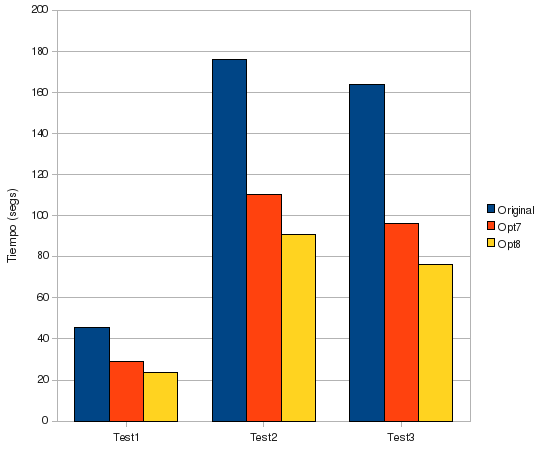
\includegraphics[keepaspectratio=true,width=.5\textwidth]{figures/opt8-perf}
\end{figure}

Las aceleraciones acumuladas sobre la versi\'{o}n original son del 91.255\%
para el primer test, 93.722\% para el segundo test y 115.730\% para el tercer
test. Sobre la versi\'{o}n Opt7 las aceleraciones son del 20.968\%, 21.608\% y
26.600\% para el primer test, el segundo y el tercero, respectivamente.

Como se puede observar, la aceleraci\'{o}n que se consigue es importante, lo que
hace que esta versi\'{o}n sea algo m\'{a}s r\'{a}pida que Opt6. El motivo es que
Utilizado la intr\'{i}nseca \texttt{\_mm\_hadd\_ps} dos veces se ahorrarn las
sumas y la intr\'{i}nseca \texttt{\_mm\_sqrt\_ss} calcula la raiz cuadrada de la
suma anterior de forma muy eficiente. Esto, a\~{n}adido al hecho de tener que
recuperar solo un valor del registro vectorial, hace que el tiempo de
ejecuci\'{o}n mejore.

\subsection{Opt9: Inlining y evitar cargas a registros vectoriales}

Viendo que el motivo principal de penalizaci\'{o}n en \texttt{pythagoras} son
los accesos a memoria y estudiando el or\'{i}gen de la mayor\'{i}a de las
llamadas a esta funci\'{o}n, se ha notado que hay parametros que se pasan a cada
llamada sin ser modificados. Este hecho provoca cargas al registro vectorial
innecesarias.

\begin{lstlisting}
    distance = pythagoras(coord[indexCoord],coord[indexCoord+1],coord[indexCoord+2],
                          x_centre,y_centre,z_centre);
\end{lstlisting}
 
Los valores \texttt{x\_centre}, \texttt{y\_centre} y \texttt{z\_centre} no
cambian a cada iteraci\'{o}n del bucle sin\'{o} que se mantienen constantes
durante muchas iteraciones. Por este motivo, haciendo inlining, se pueden
hacer cargas el registro vectorial solo cuando se modifica uno de estos valores.

\begin{lstlisting}

    centreVect = _mm_set_ps(x_centre, y_centre, z_centre, 0);
    ....
    for( atom = 0 ; atom <= num_unrolled_iters ; atom += 4 ) {
       v1 = _mm_set_ps(coord[indexCoord], coord[indexCoord+1], coord[indexCoord+2], 0);
       v1 = _mm_sub_ps(v1, centreVect);
       v1 = _mm_mul_ps(v1, v1);
       v1 = _mm_hadd_ps(v1, v1);
       v1 = _mm_hadd_ps(v1, v1);
       v1 = _mm_sqrt_ss(v1);
       _mm_store_ss(&(distance[0]), v1);
       ...
    }
\end{lstlisting}

La siguiente gr\'{a}fica muestra los tiempos de ejuci\'{o}n de la versi\'{o}n
original, de la versi\'{o}n Opt8 y de la versi\'{o}n Opt9.

\begin{figure}[ht]
   \centering
   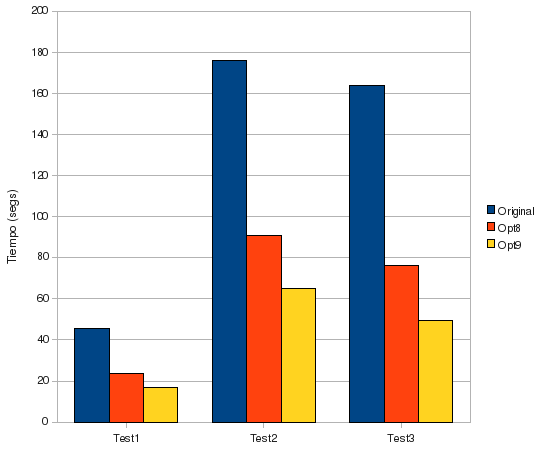
\includegraphics[keepaspectratio=true,width=.5\textwidth]{figures/opt9-perf}
\end{figure}

Las aceleraciones acumuladas sobre la versi\'{o}n original son del 166.793\% para el
primer test, 171.409\% para el segundo test y 232.882\% para el tercer test. Sobre
la versi\'{o}n Opt8 las aceleraciones son del 39.495\%, 40.102\% y 54.304\% para el
primer test, el segundo y el tercero, respectivamente.

Como se puede observar, la aceleraci\'{o}n que se consigue es muy importante. El
motivo es que se evitan muchas cargas de valores a registros vectoriales, que
son la principal fuente de p\'{e}rdida de rendimiento en c\'{o}digos vectoriales.

% vim: filetype=tex tw=75
